\documentclass{standalone}
\usepackage{tikz}
\usepackage{pgfplots}
\pgfplotsset{width=32cm,height=18cm,compat=1.3}
\pgfplotsset{every tick label/.append style={font=\Huge}}
\usepackage{filecontents}

\usetikzlibrary{patterns}

\definecolor{citrine}{rgb}{0.89, 0.82, 0.04}

\begin{document}
	\centering
		\vspace{1.5em}
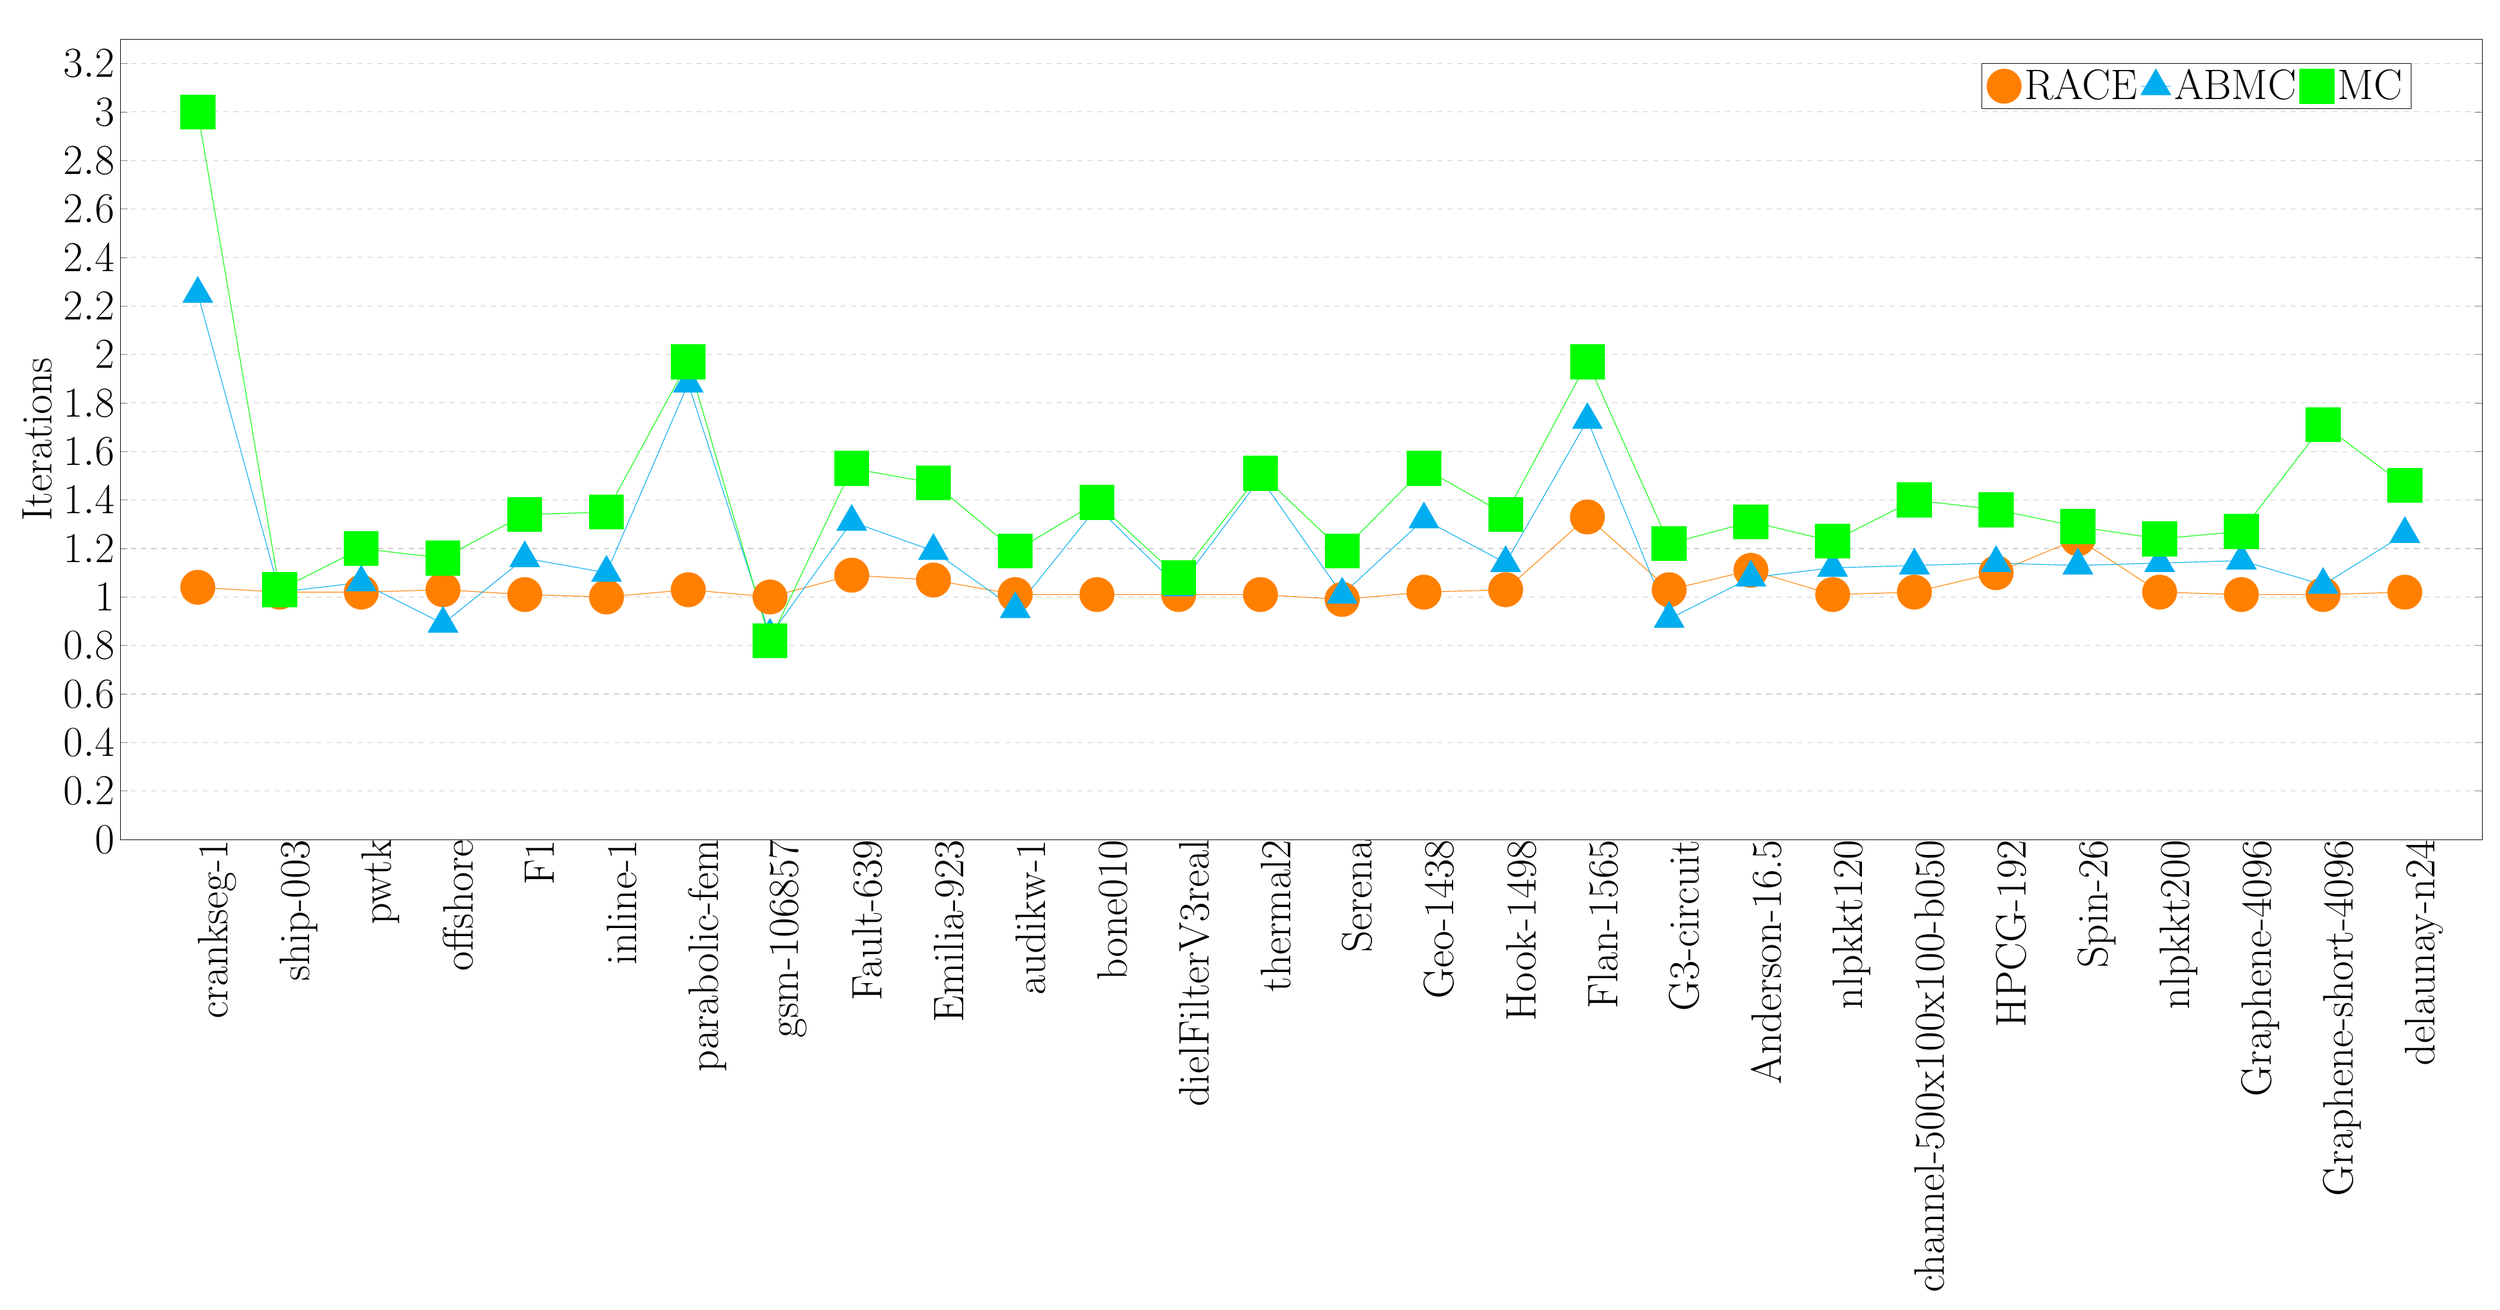
\begin{tikzpicture}
		%	\node at (13.25,15) {\LARGE{}};
			\begin{axis}[
		%	xmin=0.25, xmax=7.25,
			ymin=0, %ymax=3.25,
			xtick={1, 2, 3, 4, 5, 6, 7, 8, 9, 10, 11, 12, 13, 14, 15, 16, 17, 18, 19, 20, 21, 22, 23, 24, 25, 26, 27, 28},
		%	ytick={0,0.5,1,1.5,2,2.5,3},
			xticklabels={crankseg-1, ship-003, pwtk, offshore, F1, inline-1, parabolic-fem, gsm-106857, Fault-639, Emilia-923, audikw-1, bone010, dielFilterV3real, thermal2, Serena, Geo-1438, Hook-1498, Flan-1565, G3-circuit, Anderson-16.5, nlpkkt120, channel-500x100x100-b050, HPCG-192, Spin-26, nlpkkt200, Graphene-4096, Graphene-short-4096, delaunay-n24},
			width  = 50cm,
			height = 18cm,
			major x tick style = transparent,
			%	minor ytick={1, 5, 10, 15, 20, 25, 30 ,35,40},
			grid = minor,	
			%add_bar_commands
			ymajorgrids = true,
			grid style={dashed, gray!40},
			ylabel = {\Huge{Iterations}},
		%	symbolic x coords={Graphene-2048-2048, Graphene-4096-4096, Spin-24-24-24},
			x tick label style={rotate=90, anchor=north east, inner sep=0mm, font={\Huge}},
			tick label style={font={\Huge}},
			scaled y ticks = false,
			enlarge x limits=0.035,
			legend cell align=left,
			legend style={font=\Huge},
			legend columns=-1,
			legend style={
				%at={(1,1.05)},
				%anchor=south east,
				%column sep=1ex,
				legend pos=north east
			},
			%spl_legend_code
			title= {\Huge\scalebox{1.5}{{}}}
			]

\addplot[mark=*, mark size=10pt, mark options={orange}, draw=orange , y filter/.code={\pgfmathparse{\pgfmathresult*0.001}\pgfmathresult}] plot coordinates{(1,1040) (2,1020) (3,1020) (4,1030) (5,1010) (6,1000) (7,1030) (8,1000) (9,1090) (10,1070) (11,1010) (12,1010) (13,1010) (14,1010) (15,990) (16,1020) (17,1030) (18,1330) (19,1030) (20,1110) (21,1010) (22,1020) (23,1100) (24,1240) (25,1020) (26,1010) (27,1010) (28,1020)};
\addplot[mark=triangle*, mark size=10pt, mark options={cyan}, draw=cyan , y filter/.code={\pgfmathparse{\pgfmathresult*0.001}\pgfmathresult}] plot coordinates{(1,2250) (2,1020) (3,1060) (4,890) (5,1160) (6,1100) (7,1880) (8,840) (9,1310) (10,1190) (11,950) (12,1370) (13,1040) (14,1490) (15,1010) (16,1320) (17,1140) (18,1730) (19,910) (20,1080) (21,1120) (22,1130) (23,1140) (24,1130) (25,1140) (26,1150) (27,1050) (28,1260)};
\addplot[mark=square*, mark size=10pt, mark options={green}, draw=green , y filter/.code={\pgfmathparse{\pgfmathresult*0.001}\pgfmathresult}] plot coordinates{(1,3000) (2,1030) (3,1200) (4,1160) (5,1340) (6,1350) (7,1970) (8,820) (9,1530) (10,1470) (11,1190) (12,1390) (13,1080) (14,1510) (15,1190) (16,1530) (17,1340) (18,1970) (19,1220) (20,1310) (21,1230) (22,1400) (23,1360) (24,1290) (25,1240) (26,1270) (27,1710) (28,1460)};
	%addplot cmd

	\legend{RACE, ABMC, MC}

	\end{axis}			
\end{tikzpicture}

\end{document}

